\chapter{Introduction to Lab Activities}
\label{lab:introduction}
Software testing and test design are very important and inseparable parts of the software development process. The application of testing methods is as important as the theory of testing. This manual aims to be a supplementary document to the theoretical lectures on software testing. It can be used as an introductory guide to JUnit Jupiter API or can be followed as a text for laboratory studies. Java is chosen as the primary programming language for the exercises. Each section has two essential parts; the first one introduces the focused subject and the second one presents some exercises on the subject. Sections are designed to cover a 10-weeks semester schedule. However, some sections can be taught as two-week sections.

\section{Brief Summary of Java}
Java is an object-oriented programming language created by Sun engineers James Gosling, Mike Sheridan, and Patrick Naughton in 1991. Java programs are compiled into a special bytecode before being interpreted by Java Virtual Machine (JVM). This bytecode can be thought of as a high-level version of low-level machine languages such as Assembly. JVM interprets the bytecode and makes the system calls and other necessary operations on behalf of the running bytecode. This additional layer sometimes causes Java programs to be a little bit slower than their C/\CC~counterparts. Because of this "compilation then interpretation" stage Java can be classified as a hybrid programming language. 

One advantage of using a JVM is that every operating system has its own implementation of JVM. Therefore, the same Java program can be run in multiple operating systems without any change in the code. This is why Java is known as a platform-independent language.

\subsection{Java Terminology}
Before moving on to more complex topics, let's discuss the most common terminology of Java. Some of the below terms are discussed before and some are new.

\begin{enumerate}
    \item \textbf{Java Virtual Machine (JVM):} A written program is first converted to a low-level language called bytecode by a program called \emph{javac}. Then, JVM interprets the bytecode and makes the operation on behalf of it.
    
    \item \textbf{Bytecode:} As discussed previously, it is a low-level language model to communicate with JVM. It can be physically found in projects as files with \emph{.class} file extension.
    
    \item \textbf{Java Development Kit (JDK):} JDK is a complete development environment to develop Java programs. It contains a compiler, Java Runtime Environment (JRE), Java debuggers, Java documentations, etc.
    
    \item \textbf{Java Runtime Environment (JRE):} JRE is just an environment only capable of running pre-compiled Java programs. One cannot compile Java programs with only JRE installed. JRE includes a browser, JVM, applet supports, and plugins. To be able to run a Java program a computer should have at least JRE installed on it.
    
    \item \textbf{Garbage Collector:} Unlike C/\CC, one cannot delete objects manually in Java. This responsibility is taken care of automatically by a special program called \emph{Garbage Collector}. Garbage collector detects the objects which have not been referenced anymore and deletes them to recollect the memory occupied by them.
    
    \item \textbf{ClassPath:} The classpath is the file path where the Java runtime and Java compiler look for .class files to load. If you want to add external libraries , then you must add them to the classpath.
\end{enumerate}

\subsection{An Overview of a Hello World Program}
Java has many features. Some of them are object-oriented, multithreaded, allows sandbox execution, and the list goes on. Curious readers can find the full list on GeeksForGeeks website\footnote{\url{https://www.geeksforgeeks.org/introduction-to-java/?ref=lbp}}.

The best way to explain some syntax rules is to go through an example. Let's look at the example Java program shown in Listing \ref{lst:java-hello}.

\begin{lstlisting}[caption={Hello world example written in Java.},label=lst:java-hello]
// Demo Java program

// Importing classes from packages
import java.io.*;

// Main class
public class SomeClassName {
    // Main driver method
    public static void main(String[] args) {

        // Print statement
        System.out.println("Hello World!");
    }
}
\end{lstlisting}

The lines starting with \lstinline!//! are called \emph{comment} lines. Compilers ignore the comment lines. Comments can be single line or multiple lines. Multiple line comments start with \verb|/*| and end with \verb|*/|. e.g. \verb|/* A multiline comment */|.

The line \lstinline!import java.io.*;! means that import all the classes of \lstinline!io! package which also belongs to another package called \lstinline!java!. This is generally \textbf{not} a recommended way of importing packages.

Following the import statement, \lstinline!public class SomeClassName! defines a class. Here, \lstinline!public! is an \emph{access modifier}. It defines the places that can access to this class. Then, keyword \lstinline!class! indicates that we are defining a class with the name \lstinline!SomeClassName!. In Java, each file can have only one class (except for the inner classes) and the name of the class and the file that holds the class must be the same. Otherwise, Java compiler raises an error.

Each Java program starts from a \lstinline!static! method called \lstinline|main| which takes a \lstinline|String| array for command-line arguments. This method must be \lstinline|static| because it does not actually belong to the class which defines it and must be called externally by the JVM. In Listing \ref{lst:java-hello}, this method is defined as \lstinline!public static void main(String[] args)!. Here, the access modifier is set to \lstinline|public|. However, it is not necessary. Followed by the \lstinline|static|, the return type of the method is set to \lstinline|void|. This means that the method returns nothing after it is called which makes sense.

In Java, writing and reading operations always work on streams. In this case, by writing \lstinline{System.out.println("Hello world!");} we want to get the \lstinline|System.out| stream which is \lstinline|stdout| pseudo-file (console) and print a newline character terminated string. We can also get the \lstinline|stdin| pseudo-file to be able to read the inputs from the console by utilizing the \lstinline|System.in|.

You are now ready to expand your knowledge about Java further with this basic Java introduction. Some important resources to learn Java are \autocite{schildt2007java,schildt2010java,horstmann_2021}.

\section{Dependency Management with Maven}
Dependency management is a big part of every software development especially if multiple dependencies are involved. Each dependency can also depend on other dependencies and their specific versions. This is a huge problem because sometimes developers need to use an incompatible version as a dependency of the software they are developing which is a dependency of another dependency. These types of problems are hard to solve by humans. Because of this, various helper programs can be used. One of them is Maven, another popular one is Gradle. The list can be long for popular programming languages such as Java.

In this lab, we are going to focus on Maven. Without saying much, one can reach all the detailed information about Maven on Apache Maven Project website\footnote{\url{https://maven.apache.org/guides/getting-started/index.html}}. Let's return to the subject. Each Maven project has the same directory structure shown in Table \ref{tab:maven-dir-layout}.

\begin{table}
    \centering
    \renewcommand{\arraystretch}{1.2}
    \caption{Maven directory layout.}
    \label{tab:maven-dir-layout}
    \begin{tabular}{ll}
        \toprule
        Directory/File & Description \\
        \midrule
        \directory{src/main/java} & Application/Library sources \\
        \directory{src/main/resources} & Application/Library resources \\
        \directory{src/test/java} & Test sources \\
        \directory{src/test/resources} & Test resources \\
        \verb|target| & Output of the build \\
        \verb|pom.xml| & Description of the project \\
        \bottomrule
    \end{tabular}
\end{table}

There can be other directories in the project. A full list can be found in Apache Maven Project website\footnote{\url{https://bit.ly/34VlPvC}}. The \directory{src} directory holds the source code of the software and other resources such as images, database files, etc. The \directory{target} directory contains the output of a build. The most important file for a Maven project is the \lstinline[language={}]|pom.txt| file. This file is an Extensible Markup Language (XML) file to hold all the necessary information about the project and its dependencies. An example \lstinline[language={}]|pom.xml| file is shown in Listing \ref{lst:pom-example}.

\begin{lstlisting}[language=XML,caption={An example pom.xml file.},label=lst:pom-example]
<project xmlns="http://maven.apache.org/POM/4.0.0" xmlns:xsi="http://www.w3.org/2001/XMLSchema-instance" xsi:schemaLocation="http://maven.apache.org/POM/4.0.0 http://maven.apache.org/xsd/maven-4.0.0.xsd">
    <modelVersion>4.0.0</modelVersion>
 
    <groupId>com.mycompany.app</groupId>
    <artifactId>my-app</artifactId>
    <version>1</version>
    
    <properties>
        <mavenVersion>3.0</mavenVersion>
    </properties>
 
    <dependencies>
        <dependency>
            <groupId>org.apache.maven</groupId>
            <artifactId>maven-artifact</artifactId>
            <version>${mavenVersion}</version>
        </dependency>
        <dependency>
            <groupId>org.apache.maven</groupId>
            <artifactId>maven-core</artifactId>
            <version>${mavenVersion}</version>
        </dependency>
    </dependencies>
</project>
\end{lstlisting}

Each \lstinline[language={}]|pom.xml| file is actually an XML Schema Definition (XSD). At the top level, a project element defines the namespace information in its attributes. In the subelements, the version of the project, group id, artifact id, and properties are declared. Following the properties, a complex element called \lstinline[language={XML}]|<dependencies>| declares the dependencies of the project. There is a wide variety of elements to use inside the project. Full list can be obtained from here\footnote{\url{https://maven.apache.org/pom.html}}.

\section{Installing Eclipse and Setting up a Maven Project for Testing}
Fortunately, most of the time we do not have to deal with constructing the directory structure or writing the \lstinline[language={}]|pom.xml| file. Most Integrated Development Environments (IDE) prepare those structures with project creation wizards and automate the building tasks. You can write Java code even in the simple Notepad program. However, using an IDE greatly reduces the overhead of building and writing software. There are many great choices when it comes to IDEs. In this manual, Eclipse IDE is chosen. To install Eclipse in Windows, just go to the official website\footnote{\url{https://www.eclipse.org/downloads/}} and download the download manager and install Eclipse for Java. For Linux, just use the package manager of the distribution that you are using. Notice that, it is assumed that either OpenJDK or Oracle JDK has been already installed in your computer. Alternatively, you can install Eclipse independently from the distribution via Snap\footnote{\url{https://snapcraft.io/store}} in Linux or via Chocolatey\footnote{\url{https://community.chocolatey.org/packages}} in Windows 10 or above.

After installing Eclipse, a standard welcome screen should be opened as shown in Figure \ref{fig:eclipse-welcome}. In this screen, close the welcome tab and go to \menu{File > New > Project...}.

\begin{figure}[H]
    \centering
    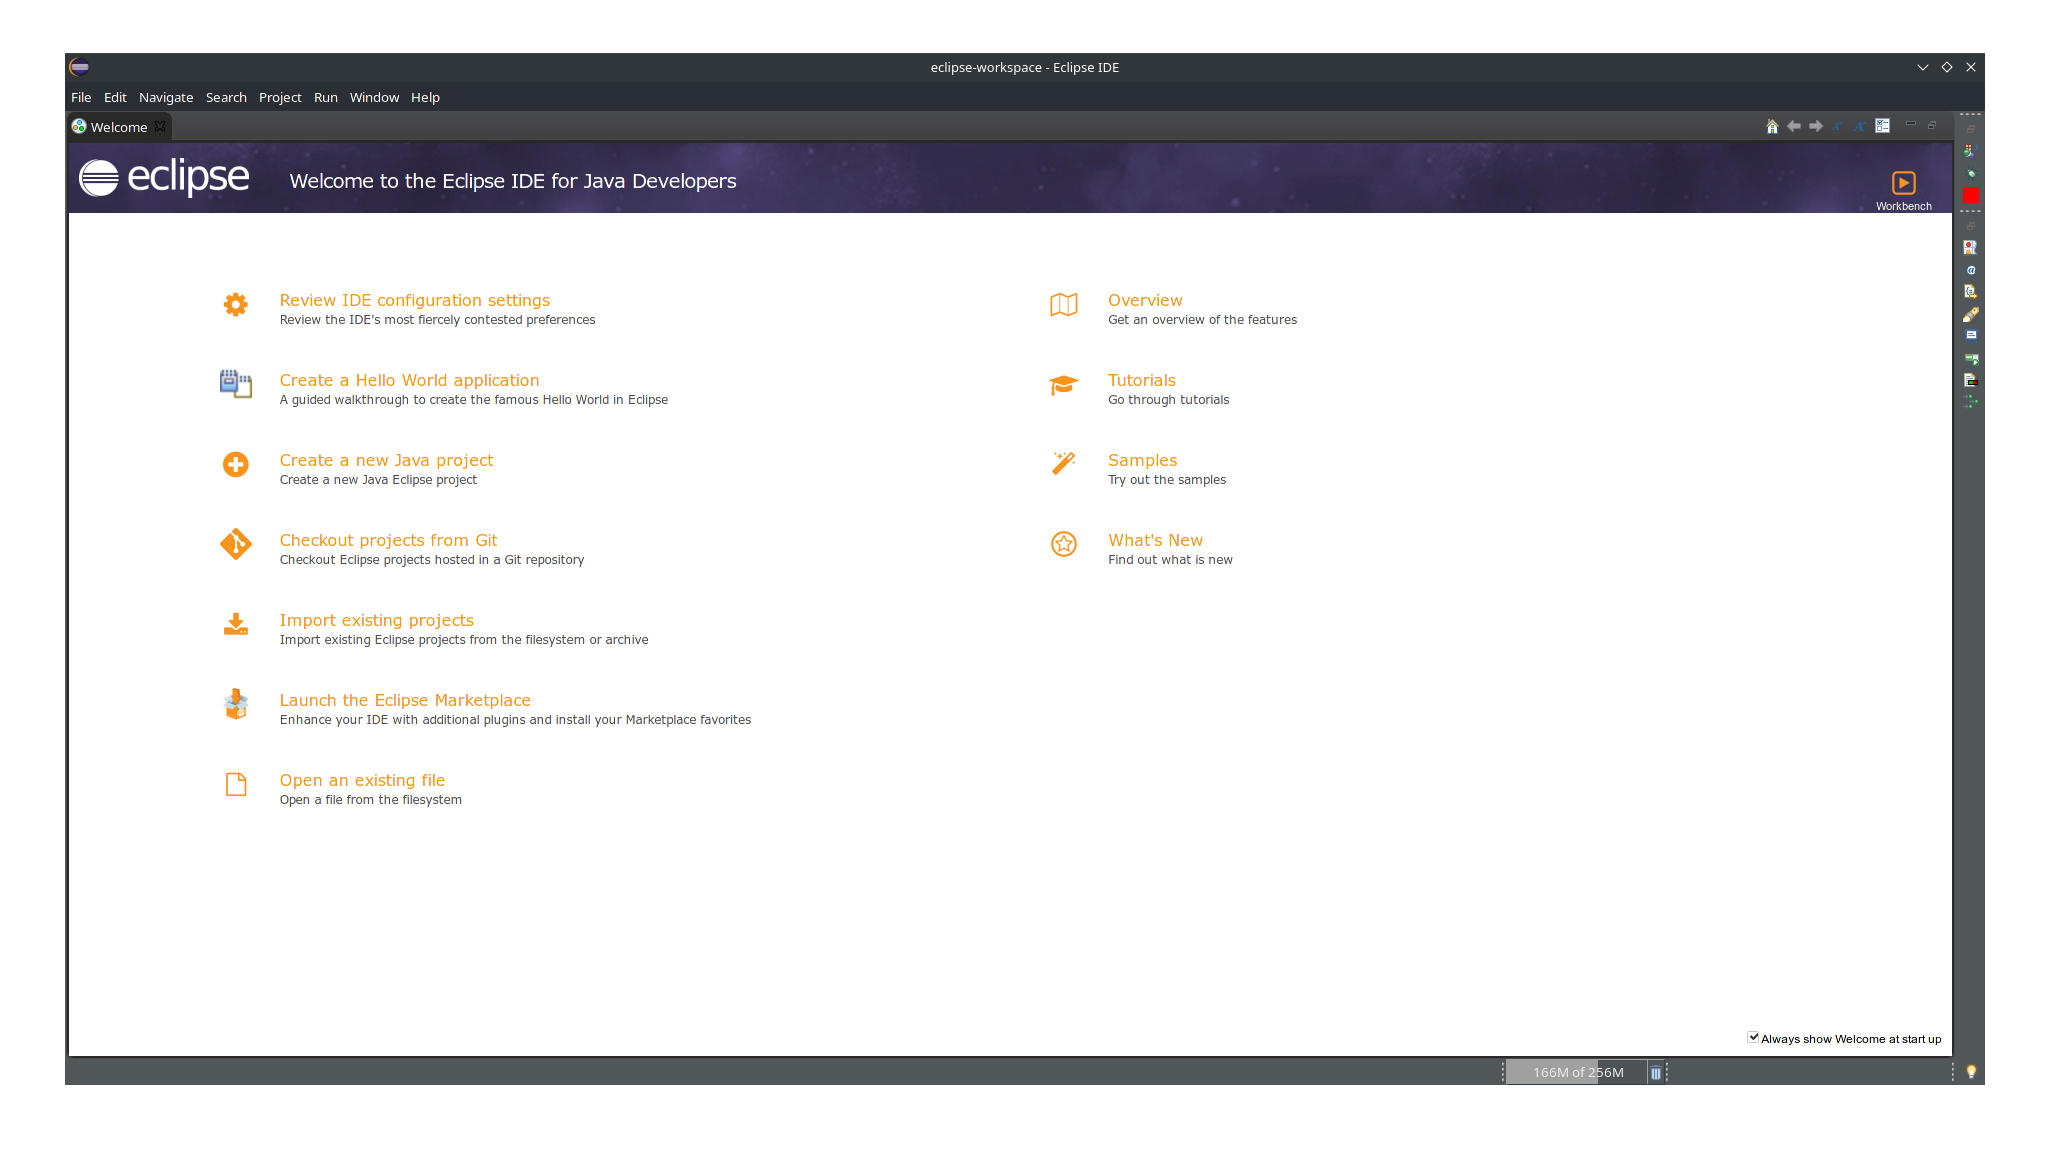
\includegraphics[width=0.95\textwidth]{images/eclipse-welcome.png}
    \caption{Welcome screen of Eclipse.}
    \label{fig:eclipse-welcome}
\end{figure}

A new dialog window should be showing up as in Figure \ref{fig:eclipse-project}. Search and choose the \emph{Maven Project}. After that, a wizard (shown in Figure \ref{fig:maven-new}) asks you a few questions about how you want to configure your new project.

\begin{figure}[H]
    \centering
    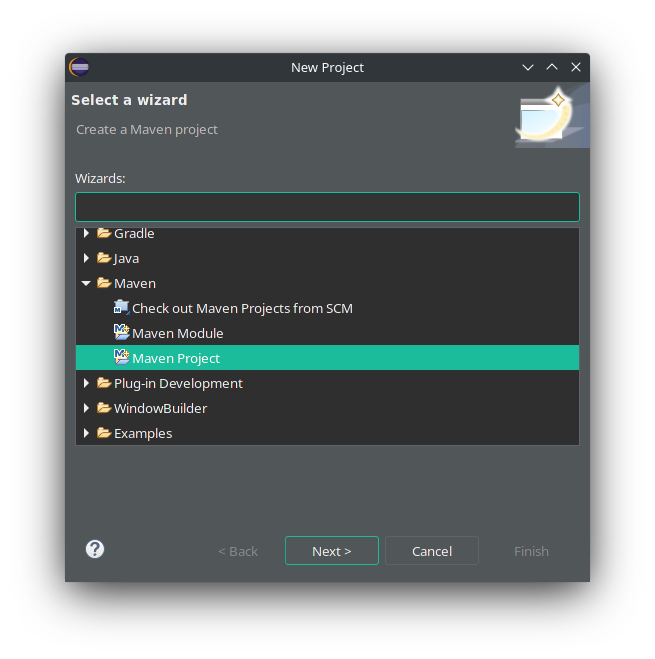
\includegraphics[width=\textwidth]{images/eclipse-project.png}
    \caption{Create a new project window.}
    \label{fig:eclipse-project}
\end{figure}

In Figure \ref{fig:maven-new}, make sure that \emph{Create a simple project} checkbox is checked. This will allow us to skip some unnecessary configuration options in the next pages. Click \keys{Next >} and you should see the dialog window shown in Figure \ref{fig:maven-app-conf}.

\begin{figure}[H]
    \centering
    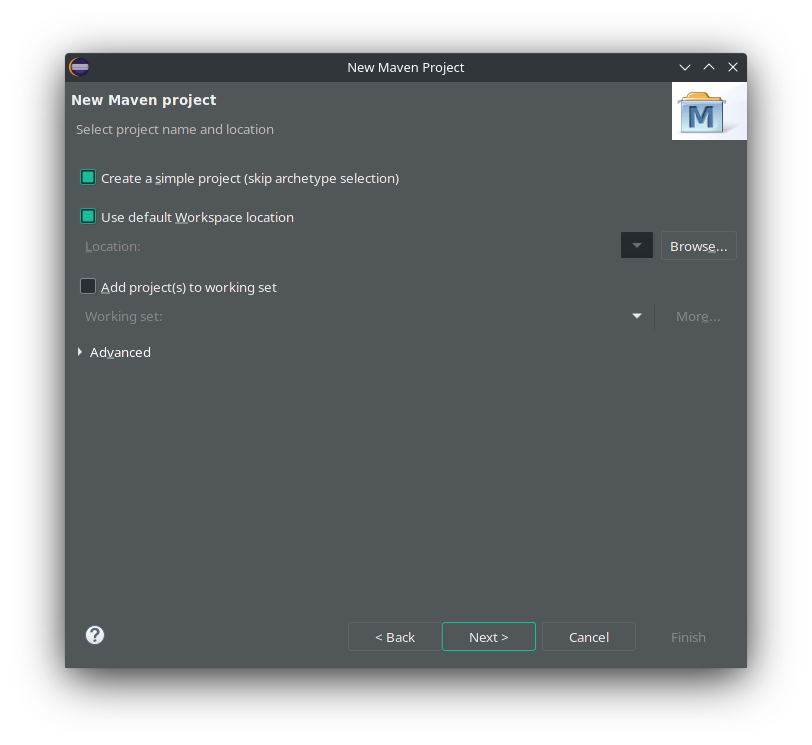
\includegraphics[width=\textwidth]{images/maven-new.png}
    \caption{Maven project wizard landing page.}
    \label{fig:maven-new}
\end{figure}

In Figure \ref{fig:maven-app-conf}, there are only two fields that must be filled before clicking to the \keys{Finish} button. The first one is the \emph{Group Id} field. Here, you should write a general package name that normally should hold all of your similar projects. For example, since we are going to write a project specifically for the SE344 lab that is offered at Atılım University, we can write something like this: \lstinline|edu.atilim.se344|. The first part, \lstinline|edu|, indicates the top-level domain as on the Internet. Then, it is followed by the company name; in this case, it is our university. Finally, followed by the name of the course. In \emph{Artifact Id}, we just give a name to our build target/executable. In this case, it is \lstinline|lab1|. When we build the project, our build target will be named like \lstinline[language={}]|lab1-0.0.1-SNAPSHOT.jar|. When you have finished filling the necessary fields, click \keys{Finish} button. The new project should be created.

\begin{figure}[H]
    \centering
    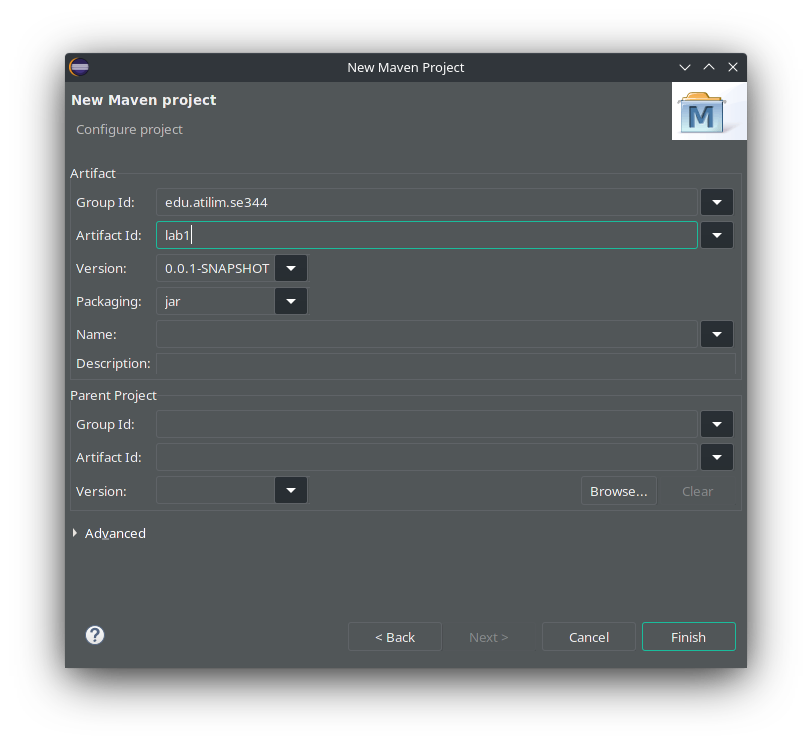
\includegraphics[width=\textwidth]{images/maven-app-conf.png}
    \caption{Maven project wizard final page.}
    \label{fig:maven-app-conf}
\end{figure}

Before moving on to the next topic, there is a small problem that we need to address. In some versions of Eclipse, Java projects have a default Java version of 1.5. This is a problem for us. Therefore, right-click to the newly created project and click \menu{Properties}. The dialog window shown in Figure \ref{fig:java-version} should be opened. Here, click \emph{Java Compiler} in the list view. Untick the checkbox starting \emph{Use compliance from execution...} and select 1.8 from \emph{Compiler compliance level} checkbox. Click \keys{Apply and Close} button when you have finished with the project properties.

\begin{figure}[H]
    \centering
    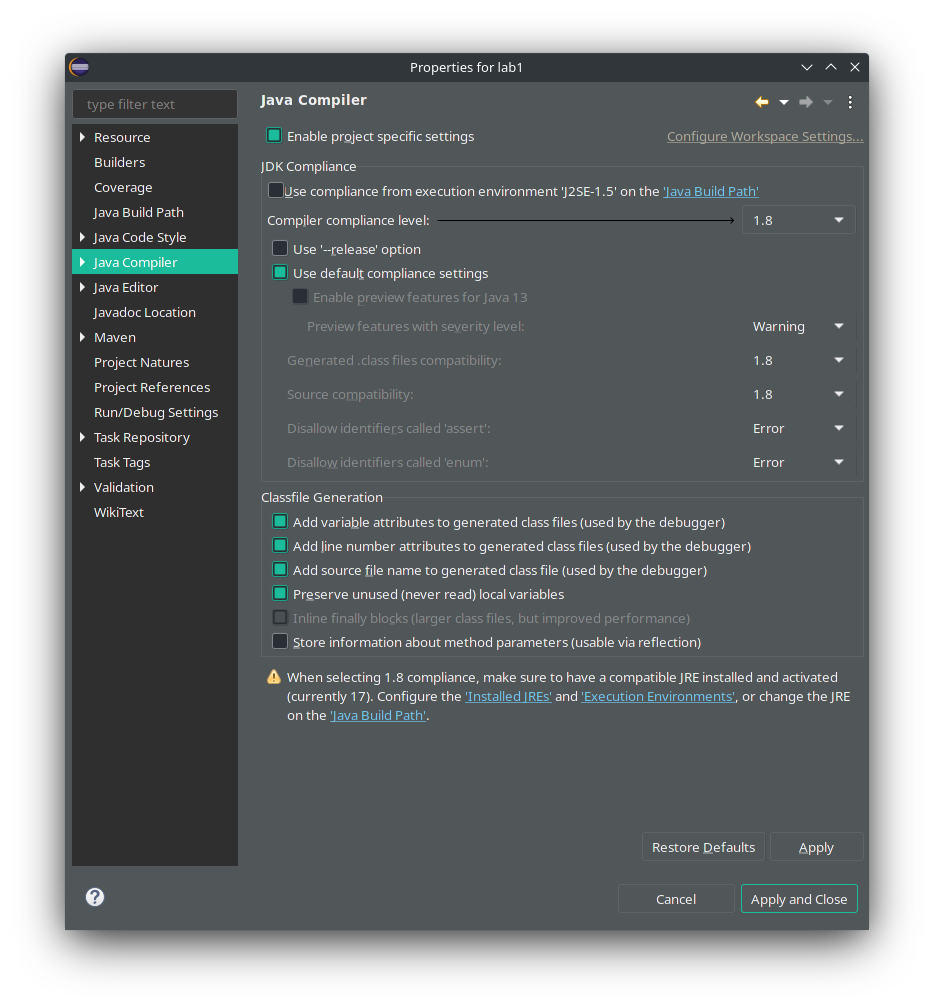
\includegraphics[width=\textwidth]{images/java-version.png}
    \caption{Java compiler properties for a Java project.}
    \label{fig:java-version}
\end{figure}

This concludes our project creation step. Now, we need to add necessary dependencies to our project's \lstinline[language={}]|pom.xml| file. In this case, there are two dependencies. They are JUnit Jupiter API and JUnit Jupiter Engine. In the next section, we are going to see how to add such dependencies to our project. Also, we need to make sure that our Maven build system is compatible with JUnit. We will add a plugin to our project to comply with JUnit.

\section{Introduction to JUnit Jupiter API}
JUnit is one of the leading unit testing frameworks for Java. It has a standard API that supplies all the necessary methods and classes for a complete test suite. In fact, it influences many other unit test frameworks in other programming languages. In Java, libraries are added to the projects by adding related \lstinline[language={}]|.jar| files to the classpath and importing them into the program. The responsibility of managing those libraries completely belongs to the developer. That is a challenging problem as stated in a previous section. Therefore, using a dependency manager is always a good idea.

In this section, we will add JUnit Jupiter API (a.k.a. JUnit 5) and Jupiter Engine to our previously created project and choose a Maven plugin version that works with the JUnit API. Remember from the previous \lstinline[language={}]|pom.xml| examples, each dependency that we want to add to our project must go to a complex element called \lstinline[language=XML]|<dependencies>|. We will use JUnit Jupiter API and Engine version 5.8.2 in this example. Go to the Maven repository website, search for the package \emph{junit}, and click the version \lstinline[language={}]|5.8.2|\footnote{\url{https://mvnrepository.com/artifact/org.junit.jupiter/junit-jupiter-api/5.8.2}}. In the middle of the page, you should see a code snippet as shown in Listing \ref{lst:pom-junit}. Copy the code snippet and paste it inside the \lstinline[language=XML]|<dependencies>| element.

\begin{lstlisting}[language=XML,caption={JUnit Jupiter API and Engine version 5.8.2 dependency elements.},label=lst:pom-junit]
<dependency>
    <groupId>org.junit.jupiter</groupId>
    <artifactId>junit-jupiter-api</artifactId>
    <version>5.8.2</version>
    <scope>test</scope>
</dependency>

<dependency>
    <groupId>org.junit.jupiter</groupId>
    <artifactId>junit-jupiter-engine</artifactId>
    <version>5.8.2</version>
    <scope>test</scope>
</dependency>
\end{lstlisting}

After adding JUnit Jupiter API, we need to indicate a specific version of Maven Surefire Plugin that works with the newest JUnit Jupiter API and Eclipse. In this case, it is the version \lstinline[language={}]|3.0.0-M5|. Add the code snippet shown in Listing \ref{lst:pom-maven-plugin} to your \lstinline[language={}]|pom.xml| file under the top-level \lstinline[language=XML]|<project>| element.

\begin{lstlisting}[language=XML,caption={A compatible Maven Surefire Plugin with Eclipse and JUnit Jupiter API v5.8.2..},label=lst:pom-maven-plugin]
<build>
    <plugins>
        <plugin>
            <groupId>org.apache.maven.plugins</groupId>
            <artifactId>maven-surefire-plugin</artifactId>
            <version>3.0.0-M5</version>
        </plugin>
    </plugins>
</build>
\end{lstlisting}

In the end, your \lstinline[language={}]|pom.xml| file should look like Listing \ref{lst:pom-future}.

\lstinputlisting[language=XML,caption={pom.xml file for future exercises.},label=lst:pom-future]{code-snippets/pom.xml}

As a final note, we prepared a Windows-based all-in-one Oracle VM VirtualBox disk image. Further information about the import process and the details of the image is given in Appendix \ref{ch:appendix-ovb-image}. It has all the packages necessary to run all the exercises in the manual. It can be directly obtained through the PCs in the lab with a 64GB USB flash drive.